\documentclass[a4paper, 10pt]{ctexart} %中文支持
\usepackage{float}              %防止浮动元素浮动
\usepackage{rotating}           %旋转图片
\usepackage{amsfonts}           %对某一些字体之支持
\usepackage{mathrsfs}           %mathscr e.g.
\usepackage[]{amsmath}          %数学公式
\usepackage{amsthm}             %定义, 定理, 证明, 例子环境的支持
%使用方法:
%\newtheorem{environment name}{caption}
%比如 \newtheorem{example}{这是例子}
%效果 \begin{example} xxx \end{example} -> 这是例子 1 xxx
%proof就不需要了
\usepackage{graphicx}           %插入图片
\usepackage[left=1.25in,right=1.25in,top=1in,bottom=1in]{geometry}   %用来排版的
\usepackage{color}            %给部分文本上色的
\usepackage{algorithm}          %写伪代码的
%\usepackage{algorithmic}       %同上
\usepackage{algorithmicx}
\usepackage{algpseudocode}
\usepackage{minted}
\usepackage{amssymb}            %用来加入一些数学符号, 比如说 $\varnothing$
\usepackage{titlesec}
\usepackage{fontspec}           %不知道用来干嘛的
\usepackage{hyperref}           %生成可跳转的书签
% -------------------------------
\setmonofont{Ubuntu Mono}       %?
\usemintedstyle{custommanni}    %设置minted插入代码的风格
\titleformat*{\section}{\huge\bfseries}             %管理title的字体和大小
\titleformat*{\subsection}{\Large\bfseries}         %bfseries就是默认的字体.
\titleformat*{\subsubsection}{\large\bfseries}
% -------------------------------
\newtheorem{theorem}{Theorem}
\newtheorem{example}{Example}
\newtheorem{definition}{Definition}
\newtheorem{lemma}{Lemma}
\newtheorem{remark}{Remark}
\newtheorem{corollary}{Comment}
\newtheorem{proposition}{Proposition}
\pagestyle{plain}
\title{chapter 8: graph theory}
\author{You \and Me}
\date{date: Yesterday}
\begin{document}
\maketitle
\tableofcontents
\newpage
\section{single-source shortest path algorithm}
\begin{corollary}
    额哦, 都没有引入, 这个ppt真的是...
\end{corollary}
\subsection{问题描述} % (fold)
\label{sub:问题描述}
简单来说, 给定一个图和图中的一个顶点, 我们要找到
这个起点到其他节点的最短路径. 只不过说, 这里可以有很多
种类别, 比如说
\begin{enumerate}
    \item 是有向图还是无向图?
    \item 是带权图还是无权图?
\end{enumerate}

我们首先处理最为简单的情况, viz. 无向无权图. 
% subsection问题描述 (end)

\subsection{一些性质} % (fold)
\label{sub:一些性质ofshortestpath}
\begin{theorem}[优化子结构]
    两个节点之间的一个最短路径, 包含着其他的最短子路径. 

    viz. 
    给定一个 $u,v$ 之间的最短路径 $p$ 
    i.e. $u \overset{p}{\leadsto}v$ ,
    对于 $p$ 上的任意两个点 $\mu ,\nu$
    , $p$ 中有一个子路径 $p'$ 使得 
    $ \mu \overset{p'}{\leadsto} \nu$
\end{theorem}
\begin{proof}[简单证明一下]
优化子结构都使用反证法, 我们说, $ \mu , \nu$ 之间
如果说, $p'$ 并不是最短的, 设最短的那个为 $p''$.
那么我们能够构造出一个比 $p$ 要短的路径:

设 $p_{1}$ 有 $u \overset{p_{1}}{\leadsto} \mu$ 然后 有 $p_{2}$: 
$\nu  \overset{p_{2}}{\leadsto} v$.
那么这样表示 $u \overset{p_{1}}{\leadsto} \mu \overset{p''}{\leadsto} \nu \overset{p_{2}}{\leadsto} v$ .
这就是一个比 $p$ 要短的路径.
\end{proof}
\begin{theorem}[三角不等式]
设 $\delta \left( u ,v\right)$ 表示 $ u ,v$ 之间的最短路径的长度 (aka权重).
那么我们有: 
\begin{align*}
\delta \left( u ,v\right) \le \delta \left( u ,v\right) + \delta \left( x,  v\right)
\end{align*}
\end{theorem}
\begin{proposition}
负圈. 如果说, 存在一个权重为负值的圈, 那么我们说, 
很可能不存在最短路径.
\end{proposition}
% subsection一些性质 (end)

\subsection{松弛} % (fold)
\label{sub:松弛}
最短路径的核心技术就是松弛, 这点比较好理解吧. 松弛的对象是两个顶点, 已知条件是
这两个顶点之间的边的权重, 以及, 当前``已知的''到两个顶点的距离.
\begin{definition}
松弛. 给定两个顶点 $ u ,v$, 松弛的操作是说, if $ d \left( u\right) + w \left( u , v\right) \le d \left( v\right)$
我们就将这个 $d \left(v\right)$ 更新为 
$d \left(u \right) + w \left( u, v\right)$ (并且可以进行记录, 记录 $v$ 的``上一个节点''应该是 $u$)
\end{definition}
我们这里稍微写一下代码
\begin{minted}{c++}
    void Relax (u,v,w(u,v)){
        if (d[v] > d[u] + w(u,v))
        d[v] = d[u] + w(u,v);
    }
\end{minted}
% subsection 松弛 (end)
\subsection{Bellman-Ford algorithm} % (fold)
\label{sub:Bellman-Ford algorithm}

% subsection Bellman-Ford algorithm (end)
\section{intro and prequisition}
\subsection{Notation}

我们研究最短路径的话, 我们必然会面对图的各种参数, 因为我们当然是在有权图上面寻找最短路径的, 如果说是那种将路径长度定义为路径所经过的节点个数的话, 正如22所讲的那样的话, 
这种就不在我们这次的研究范围内了. 于是我们给定的是 {\bf 有权, 有向图}. 

\begin{definition}
    A graph is abbreviated as $G  = \left(V, E\right)$ , 这是我们已经熟知的. 
\end{definition}

\begin{definition}
一个path记为 $p$ , 可以写为 $\left< v_{0}, v_{1}, \cdots , v_{n}\right>$ , 为了突出其终点和起点, 一个path可以记为
$$p: u \leadsto v$$
\end{definition}

\begin{definition}
$w : E \to \mathbb{R}, \left(u , v\right) \mapsto w \left(u , v\right)$ , 将权重以函数的方式写出来当然是为了严谨. 
虽然在一些人看来可能是脱裤子放屁, 但其实有很多东西的定义都是这样用函数定义的. 同时也定义了path的权重 $p \mapsto w \left( p\right) = \sum\limits_{i=1} ^{\infty} w \left( v_{i}\right)$
\end{definition}

\begin{definition}
最短路径的记号: 
\[
\delta \left(u , v\right) = 
\begin{cases}
    \min \left\{w \left(p\right) : p: u \leadsto v \right\}, &\text{ if there is a path from u to v} \\
    \infty, & \text{ otherwise}
\end{cases}
\]
\end{definition}


\subsection{some variants of single-source shortest paths}
我们目前的问题称为 single-source shortest paths. 对于有权有向图, 给定了一个source, 我们要找出从source到其他点的最短路径的大小, 以及可以求解出这个路径. 
single-source shortest paths 问题有多种变体, 当然这里只是介绍一下

\paragraph{Single-destination shortest-paths problems} % (fold)
\label{par:Single-destination shortest-paths problems}
给定一个图, 给定一个终点, 找到各个顶点到这个终点 (let's say $t$) 的最短路径. 
我们将每一个边逆向, 我们就能将其转换为一个 single-source 问题
% paragraphSingle-destination shortest-paths problems
\paragraph{single-pair shortest-path problem} % (fold)
\label{par:single-pair shortest-path problem}
给定两个顶点 $ u , v$ , 我们说, 要找到这两个顶点之间的最短路径, 
总之, 因为我们说, 优化子结构, 导致了求出了很多 $u$ 为起点 $\mu$ 
为终点的路径 ($\mu$ 是某些节点). 所以说, 我们不如直接面对single source问题.
% paragraphsingle-pair shortest-path problem (end)
\paragraph{All-pairs shortest-paths problem} % (fold)
\label{par:All-pairs shortest-paths problem}
\verb|Floyd|算法用来解决这个问题.
% paragraphAll-pairs shortest-paths problem (end)

\subsection{optimal structure of shortest paths}
rt. 最短路径具有优化子结构, 即, 
\begin{theorem}[优化子结构]
    两个节点之间的一个最短路径, 包含着其他的最短子路径. 

    viz. 
    给定一个 $u,v$ 之间的最短路径 $p$ 
    i.e. $u \overset{p}{\leadsto}v$ ,
    对于 $p$ 上的任意两个点 $\mu ,\nu$
    , $p$ 中有一个子路径 $p'$ 使得 
    $ \mu \overset{p'}{\leadsto} \nu$
\end{theorem}
\begin{proof}[简单证明一下]
优化子结构都使用反证法, 我们说, $ \mu , \nu$ 之间
如果说, $p'$ 并不是最短的, 设最短的那个为 $p''$.
那么我们能够构造出一个比 $p$ 要短的路径:

设 $p_{1}$ 有 $u \overset{p_{1}}{\leadsto} \mu$ 然后 有 $p_{2}$: 
$\nu  \overset{p_{2}}{\leadsto} v$.
那么这样表示 $u \overset{p_{1}}{\leadsto} \mu \overset{p''}{\leadsto} \nu \overset{p_{2}}{\leadsto} v$ .
这就是一个比 $p$ 要短的路径.
\end{proof}
\subsection{representation of shortest paths} 
这涉及到前面我还没看的部分, 即无向无权图的最短路径求解. 这里我们涉及 \textbf{predecessor}, 符号 $\pi  $ 的出现说明其和 \textbf{predecessor} 有关. 比如说: 
$v. \pi$ 是 $v$ 的一个前驱
%目前并不清楚这个前驱是哪里来的. 
\begin{definition}[predecessor subgraph]
$G_{\pi} = \left(V_{\pi  } , E_{\pi}\right)$ 是 predecessor subgraph , 其中 
$$V_{\pi} = \left\{v \in V : v.\pi \ne \varnothing\right\}\cup \left\{s\right\}$$ 
s 是source, 
并且
$$E _{\pi   } = \left\{ \left(v.\pi , v\right):v \in V_{\pi} - \left\{s\right\} \right\}$$
直观的来说, 就是这个 $G_{\pi}$ 是通过 $\pi$ 这个东西导出的. 那么就是, $V_{\pi}$ 就是说 $\pi$ 说明的, 能够抵达的
顶点. 然后 $E_{\pi}$ 就是一些边. 我们能够知道, 这个 $G_{\pi }$ 是一个树. 因为一个节点只有前驱. 
\end{definition}
\begin{figure}
    \centering
    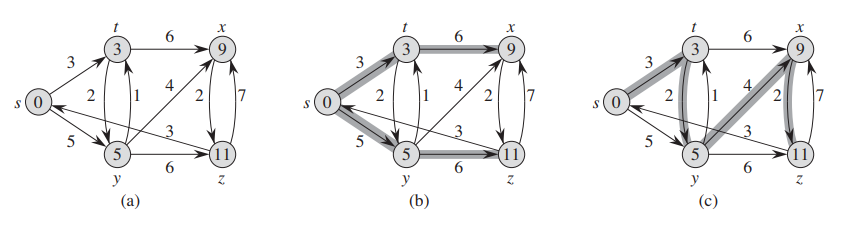
\includegraphics[scale = 0.5]{sssp4.png}
    \caption{example of relaxation}
    \label{fig:relaxation}
\end{figure}
\noindent single-source shortest paths 问题其实就是求出下面这个子图 
\\ $G'  = \left(V '  , E'\right)$ \\ $V'$ 是所有能够达到的点的集合, 即 $\delta \left(s , v\right) \ne \infty$
\\ 并且 $G'$ 是一个树, 并且这个树上的任意一个节点 $v$ , 则 $v$ 和 $s$ 之间的距离最短. 
\subsection{relaxation}
\subsubsection{initializing single source}
我们使用 $v.d$ 表示目前已知的 $v, s$ 之间的距离. 称为 \textbf{shortest path estimate}. 这时可以补充上面的 $v.\pi$ 了: $v.\pi$ 就是目前已知的 "最短路径上" $v$ 的前驱.
\begin{figure}[H]
    \centering
    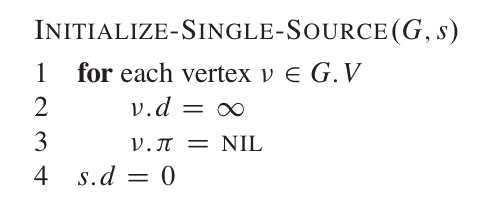
\includegraphics[scale = 0.5]{sssp2.png}
    \caption{初始化的伪代码}
    \label{iss}
\end{figure}
\subsubsection{relaxation: code and definition}
最短路径的核心技术就是松弛, 这点比较好理解吧. 松弛的对象是两个顶点, 已知条件是
这两个顶点之间的边的权重, 以及, 当前``已知的''到两个顶点的距离.
\begin{definition}
松弛. 给定两个顶点 $u ,v$, 松弛的操作是说, if $d \left( u\right) + w \left( u , v\right) \le d \left( v\right)$
我们就将这个 $d \left(v\right)$ 更新为 
$d \left(u \right) + w \left( u, v\right)$ (并且可以进行记录, 记录 $v$ 的``上一个节点''应该是 $u$)
\end{definition}
我们这里稍微写一下代码
\begin{minted}{c++}
    void Relax (u,v,w(u,v)){
        if (d[v] > d[u] + w(u,v))
        d[v] = d[u] + w(u,v);
        d.\pi= u;
    }
\end{minted}

\begin{figure}[H]
    \centering
    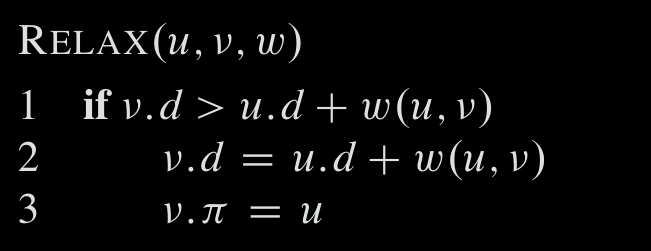
\includegraphics[scale = 0.5]{sssp3.png}
    \caption{code}
    \label{relaxation}
\end{figure}

意思即为, $u$ 到 $v$ 的一个松弛, 如果说走到 $u$ 然后走到 $v$ 的长度更短, 我们就更新 $v.d$ 目前最短路径长度; $v.\pi$ $v$ 的前驱, i.e. 更新为 $u$
而 \verb|relaxation| 只需要常数时间. 

下面是一点 quote
\begin{quotation}
Each algorithm in this chapter calls INITIALIZE-SINGLE-SOURCE and then repeatedly relaxes edges. Moreover, relaxation is the only means by which shortest
path estimates and predecessors change. The algorithms in this chapter differ in
how many times they relax each edge and the order in which they relax edges. Dijkstra's algorithm and the shortest-paths algorithm for directed acyclic graphs relax
each edge exactly once. The Bellman-Ford algorithm relaxes each edge $\left| V \right|  -1$
times.
\end{quotation}

\subsection{一些性质} % (fold)
\label{sub:一些性质}
\begin{theorem}[优化子结构]
    两个节点之间的一个最短路径, 包含着其他的最短子路径. 

    viz. 
    给定一个 $u,v$ 之间的最短路径 $p$ 
    i.e. $u \overset{p}{\leadsto}v$ ,
    对于 $p$ 上的任意两个点 $\mu ,\nu$
    , $p$ 中有一个子路径 $p'$ 使得 
    $ \mu \overset{p'}{\leadsto} \nu$
\end{theorem} 
\begin{proof}[简单证明一下]
优化子结构都使用反证法, 我们说, $ \mu , \nu$ 之间
如果说, $p'$ 并不是最短的, 设最短的那个为 $p''$.
那么我们能够构造出一个比 $p$ 要短的路径:

设 $p_{1}$ 有 $u \overset{p_{1}}{\leadsto} \mu$ 然后 有 $p_{2}$: $\nu  \overset{p_{2}}{\leadsto} v$.
那么这样表示 $u \overset{p_{1}}{\leadsto} \mu \overset{p''}{\leadsto} \nu \overset{p_{2}}{\leadsto} v$.
这就是一个比 $p$ 要短的路径.
\end{proof}
\begin{theorem}[三角不等式]
设 $\delta \left( u ,v\right)$ 表示 $ u ,v$ 之间的最短路径的长度 (aka权重).
那么我们有: 
\begin{align*}
\delta \left( u ,v\right) \le \delta \left( u ,v\right) + \delta \left( x,  v\right)
\end{align*}
\end{theorem}
\begin{proposition}
负圈. 如果说, 存在一个权重为负值的圈, 那么我们说, 
很可能不存在最短路径.
\end{proposition}
% subsection一些性质 (end)

\subsection{an outline copied from textbook}
Section 24.1 presents the Bellman-Ford algorithm, which solves the single-source
shortest-paths problem in the general case in which edges can have negative weight.
The Bellman-Ford algorithm is remarkably simple, and it has the further benefit
of detecting whether a negative-weight cycle is reachable from the source. 
Section 24.2 gives a linear-time algorithm for computing shortest paths from a single
source in a directed acyclic graph. Section 24.3 covers Dijkstra's algorithm, which
has a lower running time than the Bellman-Ford algorithm but requires the edge
weights to be nonnegative. Section 24.4 shows how we can use the Bellman-Ford
algorithm to solve a special case of linear programming. Finally, Section 24.5
proves the properties of shortest paths and relaxation stated above.

We require some conventions for doing arithmetic with infinities. We shall assume
that for any real number $a \ne -\infty$, we have $a + \infty  = \infty + a = \infty$. Also, to
make our proofs hold in the presence of negative-weight cycles, we shall assume
that for any real number $a \ne +\infty$, we have $a + \left(- \infty\right) = \left(  - \infty\right) + a =  - \infty$

All algorithms in this chapter assume that the directed graph G is stored in the
adjacency-list representation. Additionally, stored with each edge is its weight, so
that as we traverse each adjacency list, we can determine the edge weights in $O \left(1\right)$ 
time per edge.
\section{Bellman-Ford algorithm}
\subsection{an introd}
\subsection{algorithm}
\begin{figure}[H]
    \centering
    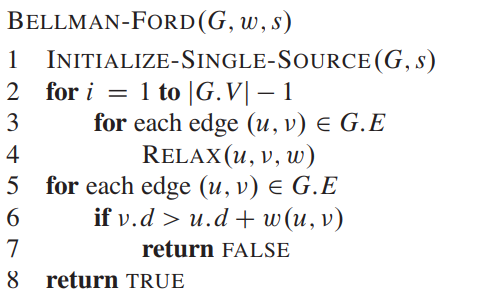
\includegraphics[scale = 0.5]{sssp5.png}
    \caption{pseus code of BF alg}
    \label{fig:bfcode}
\end{figure}
Hey maybe we can rewrite the code.
\begin{minted}[
    frame=lines,
    linenos
    ]{c++}
    boolen bellman_Ford (G , s , w) {
        for each v in V 
            d[v] = infty;
        d[s] = 0;
        for every vertex in G {
            for each edge (u,v) in E {
                relax (u,v,w(u,v));
            }
        }
        for each edge (u,v) in E{
            if (d[v] > d[u] + w(u,v)){
                return NO_SOLUTION;
            }
        }
        reture true;
    }
\end{minted}
\begin{corollary}
Note that the algorithm returns a boolen 
value. And if it returns a \verb|false|, then 
it means that the 
graph contains a negative weighted 
cycle which means that 
the solution does not 
exist. And if it returns a \verb|true| value, 
then the solution does exist. The lengths of the shortest paths
are stored in the d array.
\end{corollary}

\begin{figure}
    \centering
    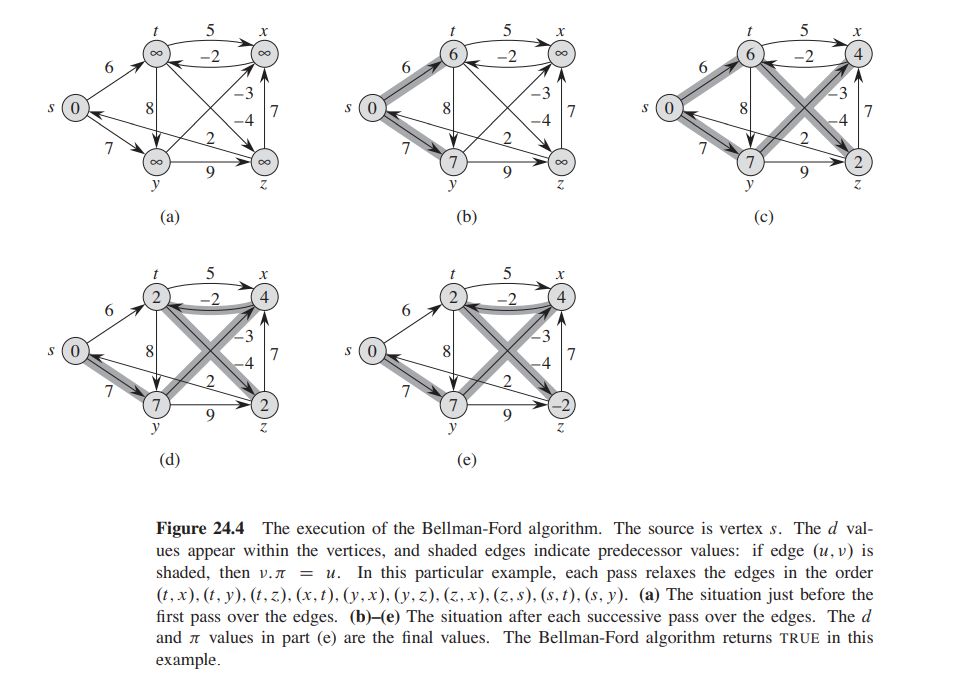
\includegraphics[scale = 0.5]{sssp6.png}
    \caption{the procedure of bellman-Ford algorithm}
    \label{fig:bellmanford}
\end{figure}
Figure~\ref{fig:bellmanford} shows a simple procedure of bellman-ford algorithm that is carried on 
a simple graph. The picture on `textbook' and those on 
ppt are the same. No pressure.
\subsection{negative weighted cycles}
The negative weighted cycles can make it that
the solution does not exist. 

So how does the algorithm detect the 
cycles?

You may see that in the algorithm, the condition
\verb|d[v] > d[u]+w(u,v)|
\subsection{the prf of algorithm}
\begin{theorem}
given $G = \left( V, E\right)$ , and a source $s$.
It is known that the $G$ has no 
negative weighted cycles.

After the \verb|line 5-9| have been 
carried out for $\left| V \right|  - 1$ 
times, for every reachable vertice $v$:
\begin{align*}
    d\left[ v \right] = \delta \left(s , v\right)
\end{align*}
\end{theorem}
\begin{proof}[proof by contradiction]
    如果说 $d\left[ v  \right] \ne \delta \left( s,  v\right)$ ,
    那么, 就有 $d\left[ v \right] < \delta \left(s ,v\right)$ because 
    $d [v] \le \delta  \left[ s, v   \right]$ 
    holds all the time.

    In the procedure of algorithm, there
    exist a vertex, let's say $u$, s.t. the following
    equality holds:
    \begin{align*}
        d[v] = d[u] + w\left(u,v\right)
    \end{align*}
    Next, use the triangle inequality.
    \begin{align*}
    d\left[ v \right] < \delta \left( s ,v\right) \le \delta \left( s,  u\right) + w \left( u, v\right) \le 
    d\left[ u  \right] + w\left( u ,v\right)
    \end{align*}
    which leads to that $d \left[ v  \right] < d\left[ u  \right] + w\left( u ,v\right)$

    Next the proof on the ppt remains unreadable. Maybe it is saying
    that very 
    \verb|for| cycle makes some shortest 
    paths' lengths are added with $1$.
\end{proof}
\begin{proof}[proof of negative weighted cycles]
    Suppose that there is a 
    negative weighted cycle
    denote as
    $c = \left< v_0 , \cdots   , v_{k} \right>$.
    It is indeed a cycle with length $k$, because $v_{0} = v_{k}$.
    We have: 
    \begin{align*}
        \sum_{i=1} ^{k} w \left( v _{i-1} , v_{i}\right) < 0
    \end{align*}
    Next we are going to prove it by contradiction. 
    If the algorithm returns true. Then 
    we have 
    \begin{align*}
        d[i] \le d[i-1] + w\left( v_{i-1} , v_{i}\right) 
    \end{align*}
    where $i =  1 , 2 , 3 \cdots , k$. Sum them up. Then 
    we have:
    \begin{align*}
        \sum_{ i=1}  ^{k} d [i  ]  & \le 
        \sum_{i = 1 } ^{k} \left( d \left[ i-1 \right] + w \left( v_{i-1} , v_{i}\right)\right)  \\
        &  = \sum_{i=1  } ^{k} d[i-1] + \sum_{i=1} ^{k} w \left( v_{i-1 }, v_{i}\right)
    \end{align*}
    Since $v_{0} = v_{k} $ , $\sum_{i=1} ^{k} d[i-1 ] = \sum_{i=1} ^{k} d [i    ]$.
    Then we have 
    \begin{align*}
        \sum_{i=1} ^{k} w \left( v_{i-1} , v_{i} \right) \ge 0 
    \end{align*}
    which contradicts to the fact that the cycle has negative weight,
    viz.
    $\sum_{i=1} ^{k} w \left( v_{i-1} , v   _{i} \right) < 0$
\end{proof}
\subsection{some blahblah}
The time complexity of Bellman-Ford algorithm is $O \left(VE\right)$ 
, which is easily to deduce. Trivial!

You can use topo ordering (whatever it calls) to 
make the algorithm more efficient.
\section{Dijkstra algorithm}
\subsection{A review}
Dijkstra algorithm requires that 
the graph has no 
negative weighted edges. Under such 
circumstance, the Dijkstra can 
reach a much more efficient algorithm.

The procedure is like prim algorithm for 
smallest spanning tree. 
\subsection{algorithm}
Figure~\ref{fig:Dijkstra} shows the algorithm
in the `textbook'. The $Q$ mentioned is a 
min-priority queue of vertices, keyed by their
$d$ values.
\begin{figure}[]
    \centering
    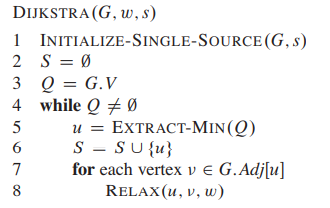
\includegraphics[scale = 0.7]{sssp7.png}
    \caption{Dijkstra}
    \label{fig:Dijkstra}
\end{figure}
\begin{corollary}
Note that 
there is a typo:
\verb|line 6| should be $S = S \cup \left\{u\right\}$
\end{corollary}
Figure~\ref{fig:dij procedure} shows a procedure 
of how Dijkstra proceed to the answer. 
\begin{figure}[]
    \centering
    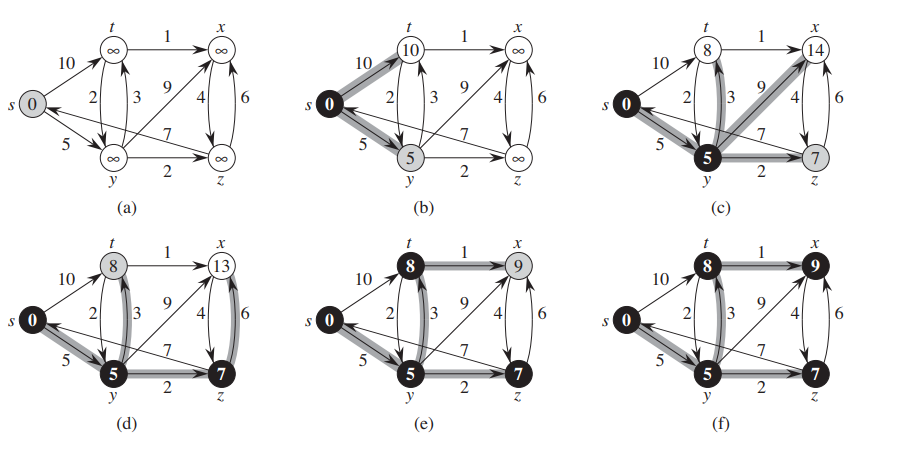
\includegraphics[scale = 0.7]{sssp8.png}
    \caption{Dijkstra procedure}
    \label{fig:dij procedure}
\end{figure}
\subsection{The prf of algorithm}
\begin{proof}
We need to prove that 
$d\left[ u   \right] = \delta \left(s, u\right)$ if $u $ is extracted 
from $Q$.

We prove by contradiction and a 
little bit induction maybe. 
If $d[u]\ne \delta \left( s, u\right) $ ,
then $d[ u]  > \delta \left( s, u\right)$

I mean, emmm, is that possible? 

Have a look at Figure~\ref{fig:prfofdij}. 
There exist $p: s \overset{p}{\leadsto} u$, $p$ is shortest. 
We say that the shortest 
to the vertices in $S$ have
been found, that is supposition from the 
induction. That is saying
\begin{align*}
    \forall  v \in S , d[v]  = \delta \left( s , u\right)
\end{align*}
Let's say that a vertex $x$ is in $S$. And let's say that 
vertex $y$ is outside of the $S$, and moreover,
$s \overset{p_{1}}{\leadsto} x \to y \overset{p_{2}}{\leadsto} u$ 
is the shortest path to $u$. 

We are going to do is to find a contradiction. How? 
The length of the shortest path is 
\begin{align*}
&     \delta \left(s , x\right)   + w\left( x,  y\right) + \delta \left( y , u\right)
= d\left[y\right] + \delta \left( y  , u\right) < d[u]
\end{align*}
which is not possible to be lower than the 
$d[u]$, because it is the shortest member amoung d's.
\begin{align*}
    d\left[ u \right] \le d[y   ]
\end{align*}
\begin{figure}[]
    \centering
    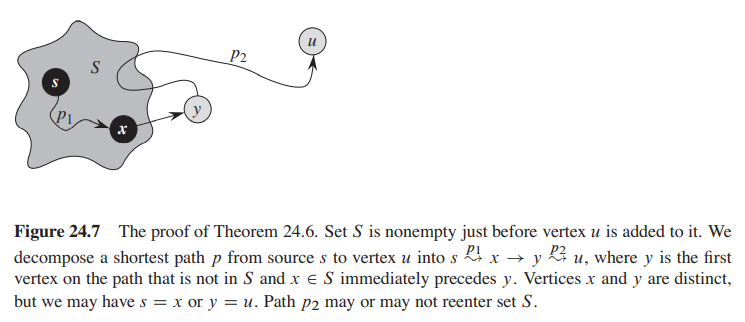
\includegraphics[scale = 0.6]{sssp9.png}
    \caption{proof of Dji}
    \label{fig:prfofdij}
\end{figure}
\end{proof}

\begin{corollary}
Here is a very crucial step: we 
assume that for the vertices in $S$,
we have
\begin{align*}
\forall x \in S,d[x ] = \delta \left( s , x\right)
\end{align*}
which is part of the induction. As for the 
complete proof, you can check out the 
proof in the `textbook', where the
author provide a 
rigorous procedure of 
proof which consist of 
three sections that are introduced in 
the former chapter of 
the book, viz. \textbf{initialization, maintainence, termination}.
\end{corollary}
\subsection{the analysis of Dijkstra algorithm}
\section{all-pairs shortest-paths algorithm}
问题描述: 
Given a weighted acyclic graph $G = \left(V , E\right)$.
Find the shortest paths of all 
pair $\left( u , v\right)$ 

Here, for the Floyd algorithm, the Graph 
contains negative weighted edge but 
does not contain the negative weighted 
cycles.

It is obvious that you 
can just carry out the 
single-source algorithm on 
each of the vertices.

BUT, what we are introducing here, 
is the Floyd algorithm, which looks 
more elegent and neat (Maybe).
\subsection{the matrix and graph}
As we have learnt in the Graph Theory, the
edges in the graph can be expressed
in the form of 
matrix. 

\begin{example}
Here is a matrix: 
\[
\begin{bmatrix}
     0 & 1 & \infty & 1 & 5\\ 
    9 &  0 & 3 & 2 & \infty \\
    \infty & \infty & 0 & 4 &\infty \\
    \infty & \infty & 2 & 0 & 3 \\
    3 & \infty & \infty & \infty & 0
\end{bmatrix}
\]
The corresponding graph is showed in Figure~\ref{fig:apsp1}
\begin{figure}
    \centering
    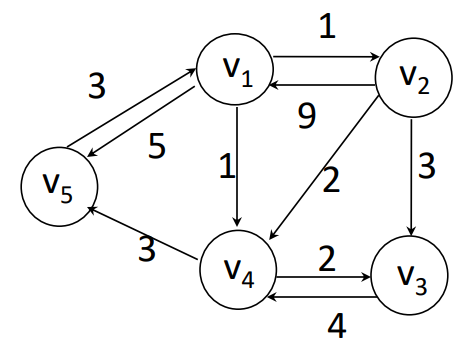
\includegraphics[scale = 0.5]{apsp1.png}
    \caption{a graph}
    \label{fig:apsp1}
\end{figure}
\end{example}
$w$ suit that 
\begin{align*}
    w_{ij} = 
    \begin{cases}
        0 & i =  j\\
        \text{weight} & i \ne j , \left( i , j\right) \in E\\
        \infty & i\ne j , \left( i , j\right) \notin E
    \end{cases}
\end{align*}
The idea of Floyd algorithm is actually dynamic programming. Here we can remind of 
how to design a dp algorithm or what need to be verified in dp.

\begin{enumerate}
    \item optimal substructure 
    \item overlapped subproblem
    \item 自底向上地计算优化解的代价并且将其保存. 并且获取构造最优解的信息.
    \item construct the solution based on the information given in the previous step.
\end{enumerate}
\subsection{前置工作}
The output of the all-pairs shortest-paths algorithms
presented here is an $n \times n   $ matrix $D = \left( d _{ij}\right)$, 
where $d _{ij}$ stands for the length of shortest path from 
$i$ to $j$. And if we are going to store the 
information of the 
shortest paths, we need not the 1-dimension 
array but another matrix, 
denoted as $\Pi = \left( \pi_{ij}\right)$ 
which is called \textbf{predecessor matrix}, where 
$\pi_{ij}$ stands for the predecessor of 
$j$ in the shortest path from $i$ to $j$.
It is clear that, if you want to 
recover the path, let's say $i \leadsto j$ from the matrix, you need to 
find $\pi_{ij}$ and then find $\pi_{i ,\pi_{ij}}$

In the previous chapter, we know that 
$\pi$ array can induce a shortest path tree $G_{\pi }$. 
Similarly, the $i$ th row of the $\Pi$ 
matrix can induce a shortest path tree.

In the textbook, the \textbf{predecessor subgraph} with respect to $i$ is defined
as $G_{\pi_{i}}$ that is the subgraph 
induced by $i$ th row of $\Pi$. 

We can list all these definitions. I mean it, that is 
good habit to do that.
\begin{definition}[the solution of apsp]
the solution value is stored in $D = d _{ij}$ and $d_{ij}$ once the algorithm 
terminates.
\end{definition}
\begin{definition}[predecessor matrix]
The information of the solution 
are store in a matrix called predecessor matrix, denoted as 
$\Pi = \left( \pi _{ij}\right)$, where $\pi_{ij}$ stands 
for the predecessor of the $j$ in the shortest
path from $i$ to $j$
\end{definition}
\begin{definition}[predecessor subgraph]
好像没什么用, 这玩意. 
\begin{align*}
    V_{\pi_{i}} = 
    \left\{ j \in V : \pi_{ij} \ne 
    \varnothing\right\} \cup \left\{i\right\}
\end{align*}
and
\begin{align*}
E_{\pi_{i}} = \left\{ \left( \pi_{ij} , j \right): j \in V_{\pi_{i}} - \left\{i\right\}\right\} 
\end{align*}
\end{definition}
\subsubsection{A chapter outline copied from the book}
Section 25.1 presents a dp algorithm based on matrix 
multiplication to solve the all-pairs shortest-paths problem.
Using the technique of 
\textbf{repeated squaring} , we can achieve a 
running time of $\varTheta  \left( V ^{3} \log  V\right)$. 

Section 25.2 presents Floyd-Warshell algorithm, which
runs in time $\Theta \left( V^3\right)$. It also 
covers the problem of finding the 
transitive closure of a directed graph. 

Finally, section 25.3 presents Johnson's algorithm, which solves the 
apsp problme in \\ $O\left( V^{2} \log  V +VE\right)$ time and 
is a good choice for large, sparse graphs.
\begin{corollary}
Unfortunately, here we are only dealing with 
the Floyd algorithm. Johnson's might looks 
attractive, but, emm, sorry.
\end{corollary}
\subsubsection{some conventions}
The capital letter like $W, L , D$ is used to 
denote a matrix. And the entries of the matrix is 
denoted as  $w_{ij}$, or $l_{ij}$, where the subscribts $i, j$ stands 
for the row and column of the entry.

Moreover, some matrices may have parenthesized superscripts, 
like $L ^{ \left( m\right) } = \left( l ^{\left(m\right)} _{ij}\right)$, 
which is, used to indicate iterates.
\subsection{An approuch}
\paragraph{a review of dp} % (fold)
\label{par:a review of dp}
Three steps: 
\begin{enumerate}
    \item characterize the structure of an optimal solution
    \item Recursively define the value of an optimal solution
    \item Compute the value of an optimal solution in a bottom-up fashion.
\end{enumerate}
% paragrapha review of dp (end)

\paragraph{the structure of a shortest path} % (fold)
\label{par:the structure of a shortest path}
The content on the `textbook' is like blahblah and so on and so on.
We just need to remember the theorem mentioned before. 

Like, give two vertices $i , j$ and then $k$ is the predecessor of 
j, then the shortest path from $i$ to $j$ can be 
expressed as $i \overset{p'}{\leadsto} k \to j$ where $p'$ is a 
subpath of $p$, and is a shortest path too. Then we have: 
\begin{align*}
\delta \left( i , j\right)  = \delta \left( i , k\right)   + w_{kj}
\end{align*}
where the length of $p$ is $m$ and the length of subpath $p'$  is $m -1$
% paragraphthe structure of a shortest path (end)

\paragraph{the recursive solution} % (fold)
\label{par:the recursive solution}
Hey, can you figure out why we mention the length of the path? 

What we are going to do is to \textbf{iterate} on the length 
of the path. 
That is, if the \textbf{shortest paths} with length \textbf{at most} $m- 1$ are known, 
we can use them to 
figure out the 
\textbf{shortest paths} with 
length \textbf{at most} $m $

These sentences above are important. Let me have a few seconds 
to digest this huge amount information.

It is actually the main idea. Not so difficult, right? 

And next step, how are we gonna iterate? Apparently, we can use 
the equation in the previous paragraph. That is 
\begin{align*}
    \delta \left( i , j\right)  = 
    \delta \left( i , k\right) + w_{kj}
\end{align*}
Oh, the solution is stored in a matrix $L$. I forget to mention.
Anyway, 
\begin{align*}
    l_{ij}^{(m)} =  
    \min_{k \in V}  \left\{ \delta \left(  i ,  k\right) + w_{kj}\right\}
\end{align*}
The initial matirx $L ^{\left( 0\right)} $ is defined as follows:
\begin{align*}
l_{ij} ^{\left(0\right)} =
\begin{cases}
    0 & \text{if } i = j \\
    \infty & \text{if } i \ne j
\end{cases} 
\end{align*} 
Apparently, the number of edges in a
shortest can not be longer than 
the $ n -1$ (there is no negative weighted cycle).
So the iteration can terminate when it reach $n-1$
% paragraphthe recursive solution (end)

\subsection{the Floyd algorithm}
It is quite surprising but we are 
now heading 
to 
the Floyd 
algorithm.

With similar approuch, but with a better
recursive method, the Floyd algorithm 
runs a little bit faster.

\paragraph{the recursive solution in Floyd} % (fold)
\label{par:the recursive solution in Floyd}
\begin{figure}
    \centering
    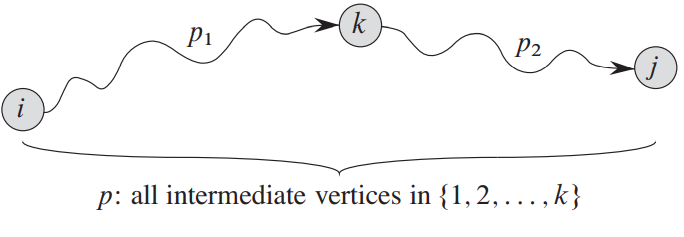
\includegraphics[scale = 0.5]{apsp2.png}
    \caption{recursive structure of Floyd}
    \label{fig:apsp2}
\end{figure}

Figure~\ref{fig:apsp2} shows the recursive structure of 
shortest paths. But here we iterate on what ? 

You can try to figure that. Moreover, what does 
`iteration' mean in the first place? 
So what does the parenthesized superscripts means here?
the $k$ in $D^{\left(k\right)}$ is actually suggesting 
the shortest paths only 
path through some vertices in 
$\left\{ 1 , 2 , \cdots , k\right\}$

Anyway, the recursive function is like
\begin{align*}
d^{\left(k\right) } _{ij} = 
\begin{cases}
    w_{ij} & k= 0 \\
    \min_{}\left\{ d^{\left(  k-1\right) }_{ij}, 
    d^{\left(k -1\right)} _{ik} + d^{(k-1)}_{kj}\right\} & 
    k \ge 1
\end{cases}
\end{align*}
% paragraph the recursive solution in Floyd (end)
\paragraph{the psedu code} % (fold)
\label{par:the psedu code}
\begin{figure}[]
    \centering
    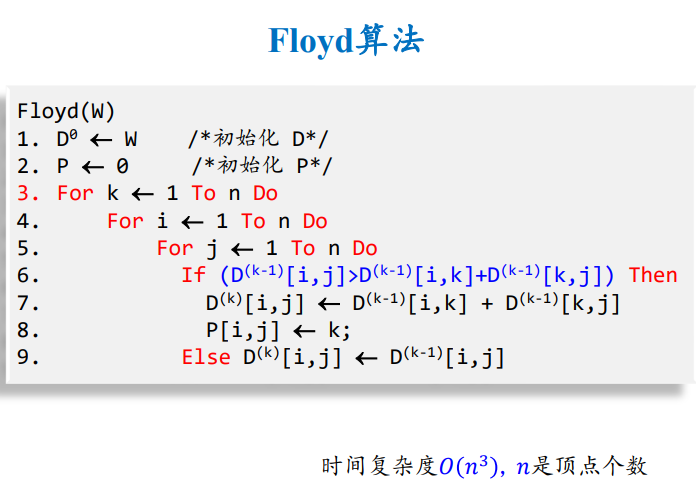
\includegraphics[scale = 0.5]{apsp3.png}
    \caption{code of Floyd}
    \label{fig:code of Floyd}
\end{figure}
The code is shown in Figure~\ref{fig:code of Floyd}
% paragraphthe psedu code (end)

\subsection{获取构造最优解的信息, 构造最优解}
We can write some codes here.
\begin{minted}[
    frame=lines,
    linenos
    ]{c++}
    int floyd (W) { // W is a matrix
        D = W;
        P = 0; // P is a matrix
        for (k = 1 to n){
            for (i = 1 to n){
                for (j = 1 to n){
                    if (D[i][j] > D[i][k]+D[k][j]){
                        D[i][j] = D[i][k]+D[k][j];
                        P[i][j] = k;
                    }
                }
            }
        }
    }
\end{minted}

The code to print
\begin{minted}[
    frame=lines,
    linenos
]{c++}
int print_path (index q , r) {
    if (P[q,r] != 0){
        print_path (q, P[q,r]);
        printf ("v", P[q,r]);
        print_path(P[q,r],r);
        return ;
    }
    esle return -1;
}
\end{minted}

\section{mf}
\subsection{some definition about flow}
2) capacity of edges 

3) flow's property

\paragraph{source and sink} % (fold)
首先我们给定一个图, 其不存在相反的边, viz. $ \left(u ,v\right) \in E \implies \left( v, u\right) \notin E $, 
其次, 这个图是一个交换图 (commute diagram) , 这是范畴论的概念. 起点称为 $ s $, source, 终点为 $ t $,  (s for sink t for terminal) 
% paragraph  (end)

\paragraph{capacity} % (fold)
存在一个权值函数 $ w $, 
使得 $ \exists \left( u ,v\right) \in E, w \left( u  , v\right) > 0 $. 这个值称为边的capacity, 
为什么起这个名字呢? 这是因为, 我们要定义一个流, 这个流的意思是, 我们从起点出发, 有一堆货物, 或者说是水, 要流到终点, 
这个流的量就是flow的值. 边的权重就是说这个边 viz. 承载流的能力. 
% paragraph (end)

\paragraph{flow's property} % (fold)
直观的讲, 我们的货物最后可别停在中间, 应流向终点, 这说明: 对于中间的节点, ``进来的''等于``出来的'', viz. 对于节点 $ v $有: 
$$ 
\sum_{}  f\left(u_{i} , v\right) = \sum_{} f \left(v , w _{i}\right) 
$$
LHS 是进的, RHS是出的. 
我们定义 $ \sum f(s , v_i) $ (或者是 $ \sum f( v_i , t) $ , 不妨证明一下为什么这两个是相等的) 为flow的值, 记为
$|f|$
% paragraph (end)

\subsection{residual networks}
我们给定一个图和一个flow, 我们下面能够自然的引出 residual networks 的定义. 记为 $ G_f' $ 这个图中的边, 表示了在 $ f $ 已经存在的情况下, 各个边的capacity. 并且存在 $ G $ 中原本没有的边, 用其相反的方向表示``减少原flow某个边的值''.

一个 flow, $f$ 是使用函数来表示的.
$$ f : E \to \mathbb R , (u,v ) \mapsto f (u,v) $$
其中 $ f(u ,v ) < c (u, v) $, 不然的话直接爆炸了.

\begin{definition}[residual graph]
$$ G_f = \{ e\in E : c(e) - f(e) > 0 \} $$
并且: 
$$ c_f \left(u ,v \right) = \begin{cases} c (u,v)  -f (u,v) & \text{if } \left(u ,v\right) \in E \\ \\ f \left( v, u\right) & \text{otherwise} \end{cases} $$
\end{definition}
\begin{corollary}
注意上面边的反向. 这说明residual 
graph上的流, 最多可以将原flow的边给
抵消掉. 
并且, residual graph的residual 
edge的数量变多了, $ E $ 中的一个边最多在 $ E_f $ 
中贡献两个. 于是有: 
$$ 
| E_f | \le 2 | E| 
$$
Trivial ! 
\end{corollary}

A flow in a residual network provides 
a roadmap for adding flow to the original
flow network. 我们现在想做的, 就是对当前这个流, 
进行一个增广. 当其足够大的
时候, 他就是最大流了 (确信). 

Observe that the residual network 
$ G_f $ is similar to a flow network 
with capacities
given by $ c_f $ . It does not satisfy 
our definition of a flow network because it may
contain both an edge $ (u,v) $ and 
its reversal $ (v,u) $. Other than 
this difference, a
residual network has the same properties 
as a flow network, and we can define a
flow in the residual network as one 
that satisfies the definition of a flow, but with
respect to capacities $ c_f $ 
in the network $ G_f $.


\subsection{augmented flow}
\begin{definition}[augmented flow]
Let's denote a flow on the residual 
graph $ G_f $ as $ f' $.
Meanwhile augmented 
flow of the original graph $ G $, which
augmented by $f'$ with the respective to
$f$, is 
denoted as $ f \uparrow f' $.
$$ 
f\uparrow f' \left( u ,v\right)= 
\begin{cases} f( u , v) + f' \left(u ,v\right) - f\left( v , u\right), &\text{ if } \left(u ,v\right) \in E \\
     0 & \text{ otherwise} 
\end{cases} 
$$
\end{definition}
Let $ G = \left(V, E\right) $ be a flow network with 
source $ s $ and sink $ t $ , and 
let $ f $ be a flow in $ G $. 
Let $ G_{f} $ be the residual network 
of $ G $ induced by $ f $ , 
and let $ f' $ be a flow in $ G_{f} $. 
Then the function $ f \uparrow f' $ 
defined in equation (上面介绍的) is a 
flow in $ G $ with value $ |f\uparrow f' | = |f| + |f'| $ 
\begin{corollary}
The conclusion that 
$\left| f \uparrow f' \right|  = \left| f \right|  + \left| f' \right| $
needs proof.
\end{corollary}
\begin{figure}
    \centering
    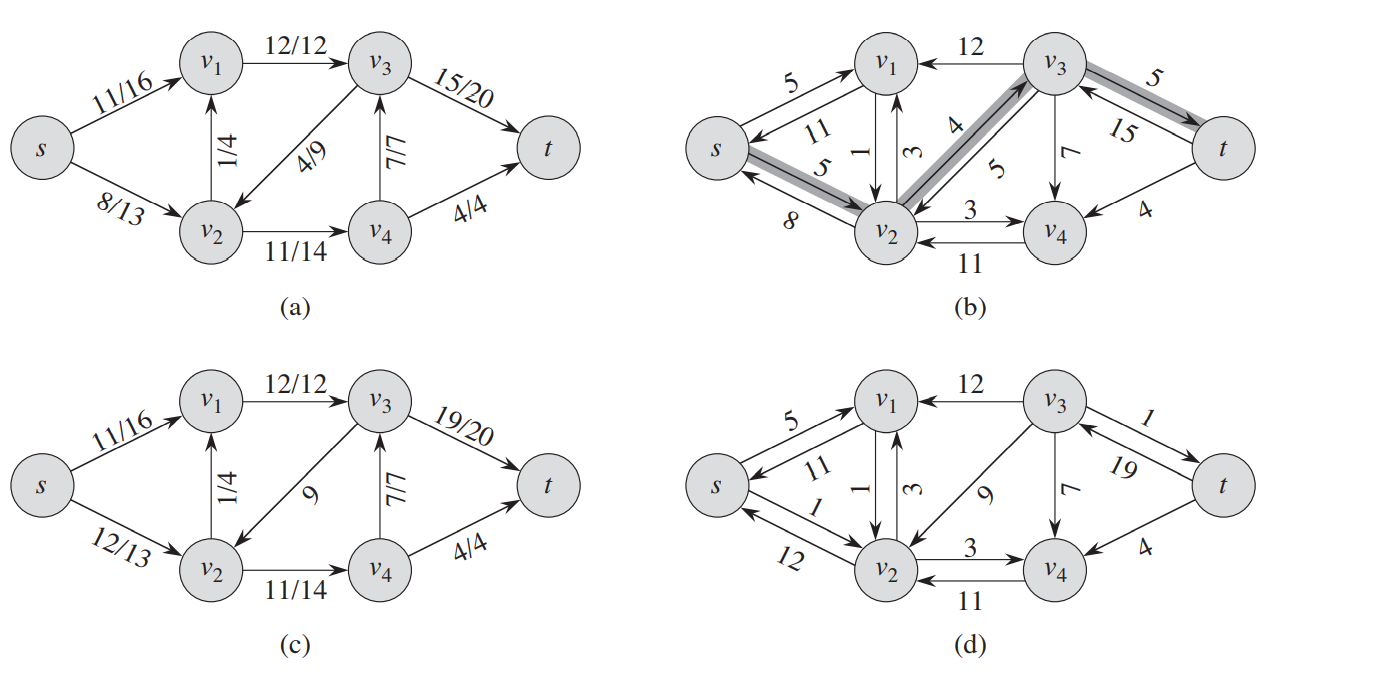
\includegraphics[scale = 0.5]{mf1.png}
    \caption{flow and augmenting path}
    \label{fig:mf1}
\end{figure}

Figure~\ref{fig:mf1} 是一个图例, 其中 (a) 是原图以及flow, (b) 是residual graph, 
然后(c)是augmented flow, (d) 是新的flow的对应的residual graph

The intuition behind this definition follows the definition 
of the residual network.
We increase the flow on $ (u,v) $ by 
$ f'(u,v) $ but decrease it by $ f'(v,u) $ because
pushing flow on the reverse edge 
in the residual network means decreasing the
flow in the original network. 

Pushing flow on the reverse edge in the residual
network is also known as \textbf{cancellation}. For example, if we send 5 crates of hockey
pucks from $ u $ to $ v $ and send 2 crates from $ v $  to $ u $, we could equivalently (from the
perspective of the final result) just send 3 creates from $ u $ to $ v $ and none from $ v $ to $ u $.
Cancellation of this type is crucial for any maximum-flow algorithm.


\subsection{augmenting paths}
Smallest residual capacity on this path is 
$ c_{f} \left(v_2 , v_3   \right) = 4 $ . We call the maximum amount 
by which we can increase the flow on each edge in 
an augmenting path $ p $ the residual capacity of $p$, given by 
$$ c_{f} \left( p\right) = \min \left\{ c _{f} \left( u  , v\right) : \left( u ,v\right) \text{ is on }p\right\} $$

\begin{lemma}[Lemma 26.2]
Let $ G = \left(V, E \right) $ be a flow network , let $ f $ be a flow in $ G $ , and let $ p $ be an augmenting path in $ G_{f} $ , Define a function $ f_{p} : V \times V  \to \mathbb{R} $ by 
$$ f _{p}  \left( u , v\right) = \begin{cases} c_{f } \left(p\right) & \text{if } \left( u,  v\right) \text{is on } p\\ 0 & \text {otherwise} \end{cases} $$
Then, $ f _{p} $ is a flow in $ G_{f} $ with value $ \left|  f_{p} \right|  = c_{f} \left(p\right) > 0 $
\end{lemma}

The following corollary show that 
if we augment $ f $ by $ f_{p} $, 
we get another flow in $ G $ whose 
value is closer to the maximum. 
Figure shows the result of augmenting 
the flow $ f $ from Figure by 
hte flow $ f_{p} $ in Figure
and Figure shows the 
ensuing residual network. 
\begin{proposition}[Corollary 26.3 ]
Let $ G = \left(V, E\right) $ be a flow network, 
let $ f $ be a flow in $ G $ , and
let $ p $ be an augmenting path in 
$ G_{f} $ . Let $ f_{p} $ be the flow defined 
above, and suppose that we augment $ f $ by 
$ f_{p} $ . Then the function 
$ f \uparrow f_{p} $ is a flow in $ G $ with value: $ \left| f \uparrow f_{p} \right| =  \left| f \right|  + \left| f_{p} \right|  > \left| f \right| $
\end{proposition}
\subsection{cut of flow networks}
How do we know Ford-Fulkerson method are 
proceed towards the 
right answer? 
The max flow min cut theorem 
tells us that 
the flow is maximum iff 
residual network contains no 
augmenting path. 
However, we shall introduce some definitions
about \textbf{cut}.

\begin{definition}[cut]
    A cut $\left( S, T\right)$ is a partition of $V$ of $G$,
    viz. $S \cup T = V$ while $S \cap T = \varnothing$
\end{definition}
With the definition of cut, we can define a \textbf{net flow} 
with the respect to the cut. 
\begin{definition}[net flow]
    Given a flow $f$, the net flow $f \left(S ,T\right)$ with the 
    respect to the cut $ \left(S ,  T\right) $
    is defined to be 
    \begin{align*}
        f \left(S , T\right) = \sum_{u \in S} 
        \sum_{v \in T}  f ( u,v)
        - \sum_{u \in S}  \sum_{ v \in T} 
        f\left( v, u\right)
    \end{align*}
\end{definition}
\begin{corollary}
Doesn't it look like the definition of 
{\bfseries flux} !?
\end{corollary}
\begin{definition}[capacity of cut]
The capacity of $ \left(S ,T\right) $ is
\begin{align*}
c \left(S , T\right) = \sum_{u \in S}  \sum_{v \in T}  c \left( u ,v\right)
\end{align*}
The minimum cut of a network is a cut 
whose capacity is minimum over all cuts 
of the network.
\end{definition}
\begin{figure}[]
    \centering
    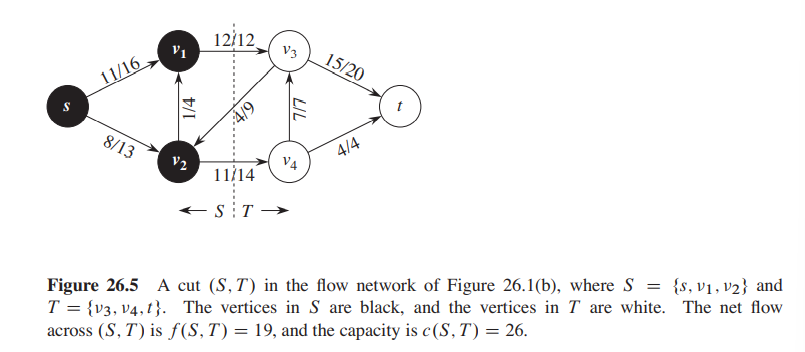
\includegraphics[scale = 0.5]{mf2.png}
    \caption{a cut}
    \label{fig:mf2}
\end{figure}
Figure~\ref{fig:mf2} shows a example of cut. 
You could try to work out the 
capacity and net flow of $(S , T)$ in the figure.

\begin{lemma}
$f$ is a flow in $G$ with source $s$ and sink $t$.
$\left(S , T\right)$ is an arbitrary cut of $G$. We 
have that 
\begin{align*}
f \left(S , T\right) =\left| f \right| 
\end{align*}
\end{lemma}
\begin{proof}
    \centering
The proof is intensionally left blank.
\end{proof}
\begin{proposition}
    For all $f$ in $G$, $\left| f \right| $ is bounded 
    above. 
\end{proposition}
\begin{proof}
    \begin{align*}
        \left| f \right|  & = f \left(S , T\right) \\
        & \le \cdots \\
        & \le \cdots \\
        & = c \left(S , T\right) \qedhere
    \end{align*}
\end{proof}
\subsection{Max flow min cut theorem}
\begin{theorem}[Max flow min cut theorem]
$f$ is a flow in $G = \left(V ,E\right)$ with source $s$ and sink 
$t$. We have three equivalent conditions:
\begin{enumerate}
    \item $f$ is at maximum.
    \item The residual graph $G_{f}$ has no augmenting paths.
    \item $\left| f \right| =  c\left(S,  T\right) $ for some cut
    $ \left( S , T\right) $ of $G$.
\end{enumerate}
\end{theorem}
\begin{proof}[proof by {\bfseries miracle}] We shall
    prove 1 to 2, 2 to 3, and then 3 to 1. We 
    shall write the proof in 
    the following enumeration.
    \begin{enumerate}
        \item[1 to 2:] The proof is easy. We shall use 
        contradictions to prove it. If there exist 
        an augmenting path then we can augment the 
        original path, so that the original one is not at 
        maximum. 
        \item[2 to 3:] If $G_{f}$ has no augmenting paths. 
        Then you can say that 
        $G_{f}$ at least have two 
        components, which allow us to 
        claim that 1. if $\left( u ,v\right) \in E$
        then $f \left( u ,v\right) $ should be $c \left( u ,v\right)$ 
        since otherwise $ \left(u, v\right)$ would be 
        in $E_{f}$. 有点难捏.
        \item[3 to 1:] which is obvious, since the
        $\left| f \right|  $ is bounded above, viz
        \begin{align*}
            \left| f \right|  \le c \left(S ,T\right) 
        \end{align*}
        and if $\left| f \right|  = c \left(S ,T\right)$ then it 
        is at maximum.
    \end{enumerate}
\end{proof}

\subsection{Ford-Fulkerson algorithm}
Finally we are arriving here. Now we shall 
introduce the Ford-Fulkerson algorithm. 

The algorithm select a augmenting path in the 
residual graph and then augment the original 
flow with the path. The procedure 
keep going until there is no augmenting path 
in the residual path, which means that 
the flow is at maximum.

Hey, maybe we can write some code.

\begin{minted}[
    frame=lines,
    linenos
]{c++}
int Ford-Fulkerson (G, s, t) {
    for each edge (u,v) in E{
        f.(u,v) = 0
    } // initialization
    while there exists an augmenting path in the residual graph{
        c_f(p) = lowest capacity in p;
        for (each edge (u,v) in p){
            if (u,v) in E   // if (u,v) in E , we augment it.
                f.(u,v) = f(u,v) + c_f(p);
            else            // if (v,u) not in E, we reduce it.
                f.(v,u) = f(v,u) - c_f(p);
        }
    }
}
\end{minted}

\begin{corollary}
Note that in the code, no steps about
the update of residual graph are written.
\end{corollary}

\subsection{the time complexity of Ford-Fulkerson algorithm}
Usually the maximum-flow problem often 
arises with integer capacities. If 
the capacities are rational numbers, 
we can make them all integer 
with certain scalar. 
And every time the path is added to 
the original flow, the value of the 
flow grow at least one. So, if $f^{*}$
stands for the 
maximum flow, the exercute times of 
adding paths is $\left| f^{*} \right| $ times.

We can use a linear time algorithm to 
find an augmenting path, but I don't know how 
to do that. Maybe, the readers can find out yourselves.
Wonderful.

Anyway, we need $O\left(E\right)$ to find a path.
So the total running  time is $O  \left(E \left| f^{*}\right| \right)$

\begin{example}
Here is an extreme example show in the Figure~\ref{fig:mf3} of how slow the Ford-Fulkerson can be.

Hey maybe you can use some greedy approuch to 
make it better. Because choosing a path with capacity $1$ instead of 
choosing one with capacity $1,000,000$ seems 
absolutely stupid.
\begin{figure}[]
    \centering
    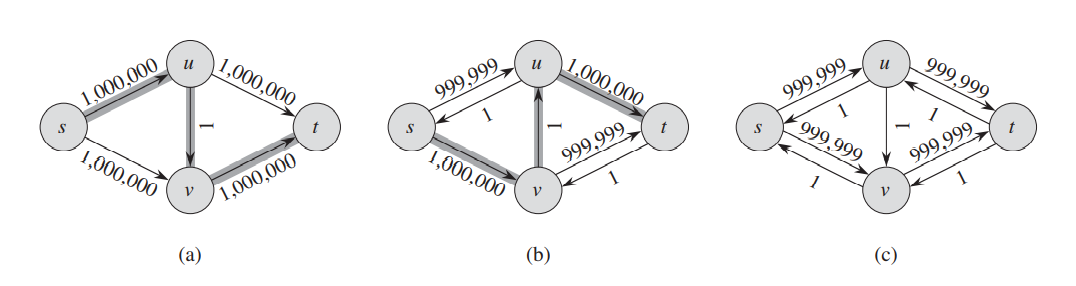
\includegraphics[scale = 0.5]{mf3.png}
    \caption{fig:an extreme example}
    \label{fig:mf3}
\end{figure}
\end{example}
\begin{corollary}
Some readers may have noticed that 
there are lots of definitions mentioned only once 
which precisely when 
it was introduced. 

They may be useless but that is not my fault.
\end{corollary}

% section start here
\section{Maximum bipartite matching}
\subsection{some definitions}
\begin{definition}[match]
Let's say that $M$ is a match of $G$. $M$ 
is subset of $E$ where for all edges in $M$, 
they have no common vertices, viz.
\begin{align*}
    \forall m_{i},m_{j} \in M, \text{他们没有公共顶点}
\end{align*}
\end{definition}

总之我们的目的是要找出匹配边, 至于说匹配是用来干什么的? 我目前还不太清楚. Anyway, 下面给出一系列的定义. 
\begin{definition}[匹配]
匹配是图的子图, 设为 $G' = \left(V' , E'\right)$, 其中 $V' = V$ , $E ' = \left\{e \in E : e \text{互不相邻}\right\}$
\end{definition}
画图就不画了, 你可以自己画一画, latex里画图好几把麻烦. 关键在于不相邻这个条件. 
\begin{definition}[最大匹配]
最大匹配是边数最多的匹配
\end{definition}
其实还有极大匹配, 就是说当前情况, 并不能再直接加边了的匹配, 但是明显, 极大匹配不一定是最大匹配. 
\begin{definition}[完美匹配]
每一个顶点都是 $M$ 中的边的顶点.
\end{definition}
\begin{definition}[匹配边, 非匹配边]
$E' $ 即为匹配边, $E - E' $ 为非匹配边.
\end{definition}
\begin{definition}[交错路径]
如果说 $p = \left< e_1, \cdots  , e_{n}\right>$ 中 $e_{i}$ 交错地是匹配边和非匹配边, i.e.  $e_{i}$ 是匹配边, 那么 $e_{i+1}, e_{i-1}$ 都是非匹配边, 那么称这个路径是交错路径.
\end{definition}
\begin{definition}[增广路径]
如果说一个路径, 是交错路径, 并且非匹配边多于匹配边, 那么这个路径是增广路径.

{\bfseries 进一步说, 增广路径不是一个圈, 并且, 两端一定是非匹配边.}
\end{definition}

如果我们已知一个增广路径, 我们可以将其增广, viz. 将他们匹配和非匹配的身份调换, 这样匹配边数量加一.
\subsection{algorithm}
对于一个二部图, 我们有定理: 
\begin{theorem}
一个匹配是最大匹配 $\iff $ 其没有增广路径.
\end{theorem}
那么这个定理足以证明下面算法的正确性:
\begin{description}
    \item[1] 找到augmenting路径.\footnote{一个不和匹配边相邻的边, 也能称为augmenting路径} 
    \item[2] 将augmenting路径augment. 
    \item[3] 直到不存在augmenting路径.
\end{description}
总之, 我们使用ppt上的语言将其再描述一遍:
\begin{enumerate}
    \item 令 $M$ 为空
    \item 找到一个增广路径 $P$, 通过将其取反, 得到更大的匹配
    \item 重复步骤 $2$, 直到我们找不到增广路径.
\end{enumerate}
\subsection{application}
\begin{example}
现在要给 $4$ 个工人 $A,  B, C , D$ 分配任务. 每一个工人
可以完成特定的一些任务, 但是最多只能够接受一个任务, 
总共有 $4$ 个任务, 每个任务只能分配给一个工人. 
请问最多能够分配多少个任务给工人. 

我们用 Table~\ref{tab:tab1} 来表示这些工人能做什么任务.
\begin{table}
    \centering\begin{tabular}{||c c c c c||}
        \hline 
        & 任务1 & 任务2 &任务3  &任务4\\ [0.5ex]
        \hline \hline
        A &  1 & 0 & 1 & 0 \\
        \hline 
        B & 1 & 0 & 0 &  0 \\
        \hline 
        C & 1 & 1 & 0 & 0 \\
        \hline 
        D & 0 & 0 & 1 & 1 \\
        \hline
    \end{tabular}
    \caption{1 表示能成, 0 表示不能成}
    \label{tab:tab1}
\end{table}
\end{example}

总之, 这个问题就能够转化为一个二部图求解最大匹配的问题, 
工人之间没有连线, 任务之间也没有连线, 所以是二部图. 
而连线代表的是任务分配. 就是说, 我们将某个工人和
某个任务之间连了起来, 则说明我将这个任务分配了给他.

因为一个工人不能同时做两份工作, 也不能两个工人同时做
一个任务, 那么
我们这里就是求一个最大匹配. 
\end{document}